\section{Uvod}
\label{sec:uvod}

Funkcionalna paradigma danas predstavlja jedan od najznačajnijih stilova jezika i u širokoj je upotrebi kako u akademskim tako i u industrijskim krugovima. Funkcionalna paradigma se zasniva na matematičkim funkcijama, eliminiše bočne efekte i tako umnogome olakšava dokazivanje korektnosti programa. Džon Bakus je 1977. godine dobio Tjuringovu nagradu za doprinos u razvoju jezika FORTRAN, a u govoru, prilikom prijema nagrade, izneo je niz argumenata zbog čega su funkcionalni jezici bolji od imperativnih. Da bi potkrepio svoje tvrdnje predstavio je funkcionalni jezik FP.

Prilikom izučavanja svake programske paradigme, velika pažnja posvećuje se prevodenju izvornog koda do izvršnog koda, to jest kompajliranju(eng. \emph{compile}). Kompajliranje funkcionalnih jezika, zbog njihovog dizajna, ima posebna svojstva. U ovom radu fokus će biti na procesu transformacije od izvornog koda do mašinskog jezika, stoga za bolje razumevanje poželjno je da se čitaoc dobro upozna sa nekim osnovnim elemtima funkcionalnog jezika koje su date u radu \cite{ajzenhamer} . Detaljno ce biti opisane 3 glavne faze : Frontend, Middle end i backend. Radi konkretnosti, fokusirali smo se na Glazgov Haskel Kompajler (eng. Glasgow Haskell Compiler(GHC)) \cite{GHCxx}, ali ističemo da sve što navedemo u ovom radu se odnosi i na bilo koji kompajler funkcionalnih jezika, a možda i na kompajliranje drugih jezika. GHC preuzima ovu ideju “kompilacije transformacijom” (eng. \emph{compilation by transformation}) pokušavajući da što više izrazi proces kompilacije u obliku programskih transformacija, iz razloga što automatke transformacije znatno poboljšavaju performanse generisanog koda. U ovom radu prikazaćemo primenu transformacione tehnike kroz GHC. 

\section{Uvod u Haskel i GHC} 

Haskel je funkcionalni jezik opšte namene, koji sadrži mnoge inovacije u dizajnu programskih jezika. Haskel podržava funkcije višeg reda (eng. \emph{ higher-order functions}), ne-striktnu semantiku, statički polimorfizam, korisnički definisane algebarske tipove, prepoznavanje šablona (eng. \emph{ pattern-matching}), rad sa listama. Razvijen je kroz sistem modula kao proširenja programskog jezika. Poseduje veliki skup primitivnih tipova uključujući liste, nizove, cele brojeve različitih namena i dužina, realne brojeve. Može se reći da je Haskel završetak dugogodišnjeg rada i istraživanja na ne-striktnim funkcionalnim jezicima \cite{Has10}. Baš zbog ovih specijalnih odluka u dizajnu, problem kompilacije kod Haskela, a i funkcionalnih jezika uopšte se smatra veoma teškim.   

GHC se uobičajno tretira kao standardna implementacija Haskela, na kojoj se baziraju i druge implementacije. Razvijan je počev od 1989. godine. GHC je pisan u Haskelu – kompajler sadrži 227,000 linija k\^{o}da (uključujući komentare), a biblioteke (moduli) sadrže 242,000 linija k\^{o}da (uključujući komentare).
Sastavni deo svakog kompajlera za funkcionalni jezik čini i run-time sistem. Za GHC, run-time sistem je pisan u C-u i sadrži 87,000 linija k\^{o}da. Tekuću verziju kompajlera razvijalo je 23 programera (eng. developers) sa preko 500 priloga (eng. commits) \cite{StanfordGHC}.  


Celokupni rad kompajlera se sastoji iz tri faze:
\begin{enumerate}
	\item Prva faza (eng. \emph{Frontend}) čini pretvaranje izvornog k\^{o}da pisanog u Haskelu, u takozvani Core jezik (eng. \emph {Core language}). U ovoj fazi, kompajler napisan u Haskelu, vrši analizu izvornog k\^{o}da, pravi odgovarajuće drvo izvođenja, realizuje leksičku i sintaksnu analizu, proveru tipova i kao izlaz daje k\^{o}d sa veoma redukovanim skupom instrukcija, koji zahteva Core. Više o ovoj fazi može se naći u poglavlju \ref{sec:frontend}.
	\item Druga faza (eng. \emph {Middle End}) – izlazni k\^{o}d iz prethodne faze – međujezik (eng. \emph {intermediate language}) se dodatno optimizuje, i to kroz niz transformacija. Rezultat rada Core-a se dobija u Core obliku. Na taj način, sledeće etape transformacije k\^{o}da tačno znaju kakve konstrukcije im se mogu naći na ulazu.  Više o ovoj fazi može se naći u poglavlju \ref{sec:middle}.
	\item Treća faza (eng. \emph {Backend}) obuhvata generisanje k\^{o}da. Core-ov k\^{o}d iz prethodne faze postaje ulaz u STG-mašinu (eng. \emph {Spineless Tagless G-machine}). Rezultat rada STG-mašine se grana u tri toka. Prvi tok podrazumeva prevođenje u izvorni mašinski k\^{o}d. 
	
	Drugi tok podrazumeva korišćenje LLVM-a (eng. \emph{Low-Level Virtual Machine}) za dobijanje optimizovanog k\^{o}da pomoću ove virtualne mašine.
	
	Treći tok koristi jezik C-\,- za dobijanje izvršnog k\^{o}da. Više o ovoj fazi može se naći u poglavlju \ref{sec:backend}.
\end{enumerate}

Razvojne etape pravljenja izvršnog k\^{o}da mogu se videti na slici \ref{fig:razvojneEtaple} preuzetoj sa \cite{StanfordGHC}.

\begin{figure}[h!]
	\begin{center}
		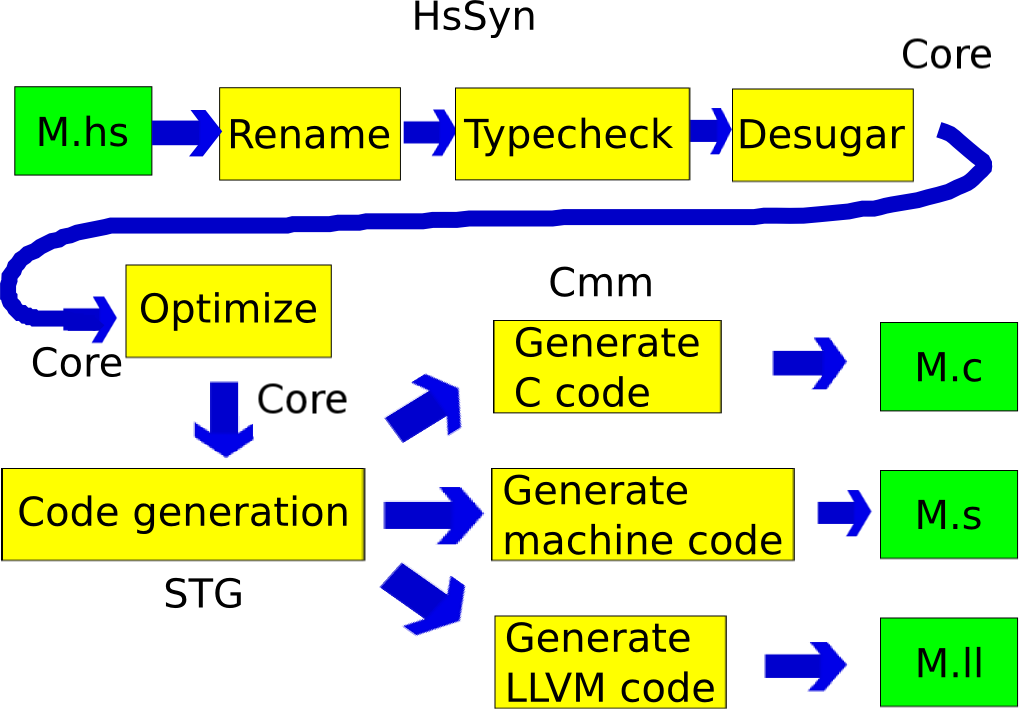
\includegraphics[scale=0.30]{resources/razvojneEtape.png}
	\end{center}
	\caption{Razvojne etape pravljenja izvršnog k\^{o}da}
	\label{fig:razvojneEtaple}
\end{figure}